\documentclass[utf8, russian, a3paper, landscape]{eskdgraph}
\usepackage{graphicx}

% Нумератор
\newcommand{\No}{\textnumero}

% Настройки штампа
\ESKDgroup{Кафедра ЭВМ\\ИВТб-2301-05-00}
\renewcommand{\ESKDcolumnXfIIname}{}
\renewcommand{\ESKDcolumnXfIIIname}{}
\renewcommand{\ESKDcolumnXfIVname}{Пров.}
\renewcommand{\ESKDcolumnXfVname}{Консул.}
\ESKDauthor{Черкасов}
\ESKDcolumnXIfII{Зинин}
\ESKDcolumnXIfIV{Коротких}
\ESKDcolumnXIfV{Мельцов}
\ESKDapprovedBy{Долженкова}
\ESKDsignature{}

\makeatletter
\renewcommand{\ESKDdrawStampI}{%
  \put(\ESKDltu{\ESKDstampX},\ESKDltu{\ESKDstampY}){%
    \usebox{\ESKD@stamp@i@box}}%
  \put(\ESKDltu{\ESKDstampX},\ESKDltu{\ESKDstampY}){%
    \ESKD@stamp@i@var}%
  \put(\ESKDltu{\ESKDstampX},\ESKDltu{\ESKDstampY}){%
    \begin{picture}(0,0)(0,0)
      \put(67, 41){\parbox[b][13mm][c]{106mm}{\centering\ESKDfontVII\ESKDtheSignature}}
    \end{picture}}%
}

\renewcommand{\ESKDdrawColumnXXVI}{%
  \ifESKD@column@xxvi@portrait%
    \setlength{\ESKD@tmpdima}{\ESKDframeX+\ESKDframeW-14mm}%
    \setlength{\ESKD@tmpdimb}{\ESKDframeY+\ESKDframeH}%
    \put(\ESKDltu{\ESKD@tmpdima},\ESKDltu{\ESKD@tmpdimb}){%
      \begin{turn}{270}%
        \usebox{\ESKD@column@xxvi@box}%
        \begin{picture}(0,0)(0,0)
          \put(1,13){\begin{turn}{180}\parbox[b][12mm][c]{68mm}{%
            \centering\ESKDfontV\ESKDtheSignature}\end{turn}}
        \end{picture}%
      \end{turn}}%
  \else%
    \setlength{\ESKD@tmpdima}{\ESKDframeY+\ESKDframeH-14mm}%
    \put(\ESKDltu{\ESKDframeX},\ESKDltu{\ESKD@tmpdima}){%
      \usebox{\ESKD@column@xxvi@box}%
      \begin{picture}(0,0)(0,0)
        \put(1,13){\begin{turn}{180}\parbox[b][12mm][c]{68mm}{%
          \centering\ESKDfontV\ESKDtheSignature}\end{turn}}
      \end{picture}}%
  \fi}

% Переопределяем изменчивые поля штампа, чтобы они рисовались на всех листах
\renewcommand{\ESKD@stamp@i@var}{%
\begin{picture}(0,0)(0,0)
  % Выводим название и другие атрибуты на всех листах
  \put(67, 16){\parbox[b][23mm][c]{66mm}{\centering\ESKDfontV\ESKDtheColumnI}}
  \put(67, 1){\parbox[b][13mm][c]{66mm}{\centering\ESKDfontV\ESKDtheColumnIII}}
  \put(135, 26.3){\makebox[5mm]{\ESKDfontIII\ESKDtheColumnIVfI}}
  \put(140, 26.3){\makebox[5mm]{\ESKDfontIII\ESKDtheColumnIVfII}}
  \put(145, 26.3){\makebox[5mm]{\ESKDfontIII\ESKDtheColumnIVfIII}}
  \put(151, 21){\parbox[b][13mm][c]{15mm}{\centering\ESKDfontIII\ESKDtheColumnV}}
  \put(168, 21){\parbox[b][13mm][c]{16mm}{\centering\ESKDfontIII\ESKDtheColumnVI}}
  \put(137, 1){\parbox[b][13mm][c]{46mm}{\centering\ESKDfontV\ESKDtheColumnIX}}
  
  \ifESKD@enable@column@viii
    \put(155, 16.3){\makebox[30mm]{\ESKDfontIII%
      \ifESKD@twoside\ESKDcolumnVIIItwosideName\else\ESKDcolumnVIIIname\fi%
      \ 1}}
  \fi
  
  \ifESKD@enable@column@vii
    \put(135, 16.3){\makebox[20mm]{\ESKDfontIII%
      \ifESKD@twoside\ESKDcolumnVIItwosideName\else\ESKDcolumnVIIname\fi\ 1}}
  \fi
\end{picture}}
\makeatother

\begin{document}
\ESKDstyle{formI}

\gdef\ESKDtheSignature{ТПЖА.090301.838-01 ДПЛ}
\gdef\ESKDtheTitle{Схема взаимодействия системы с пользователем}
\begin{center}
  \vspace*{10mm}
  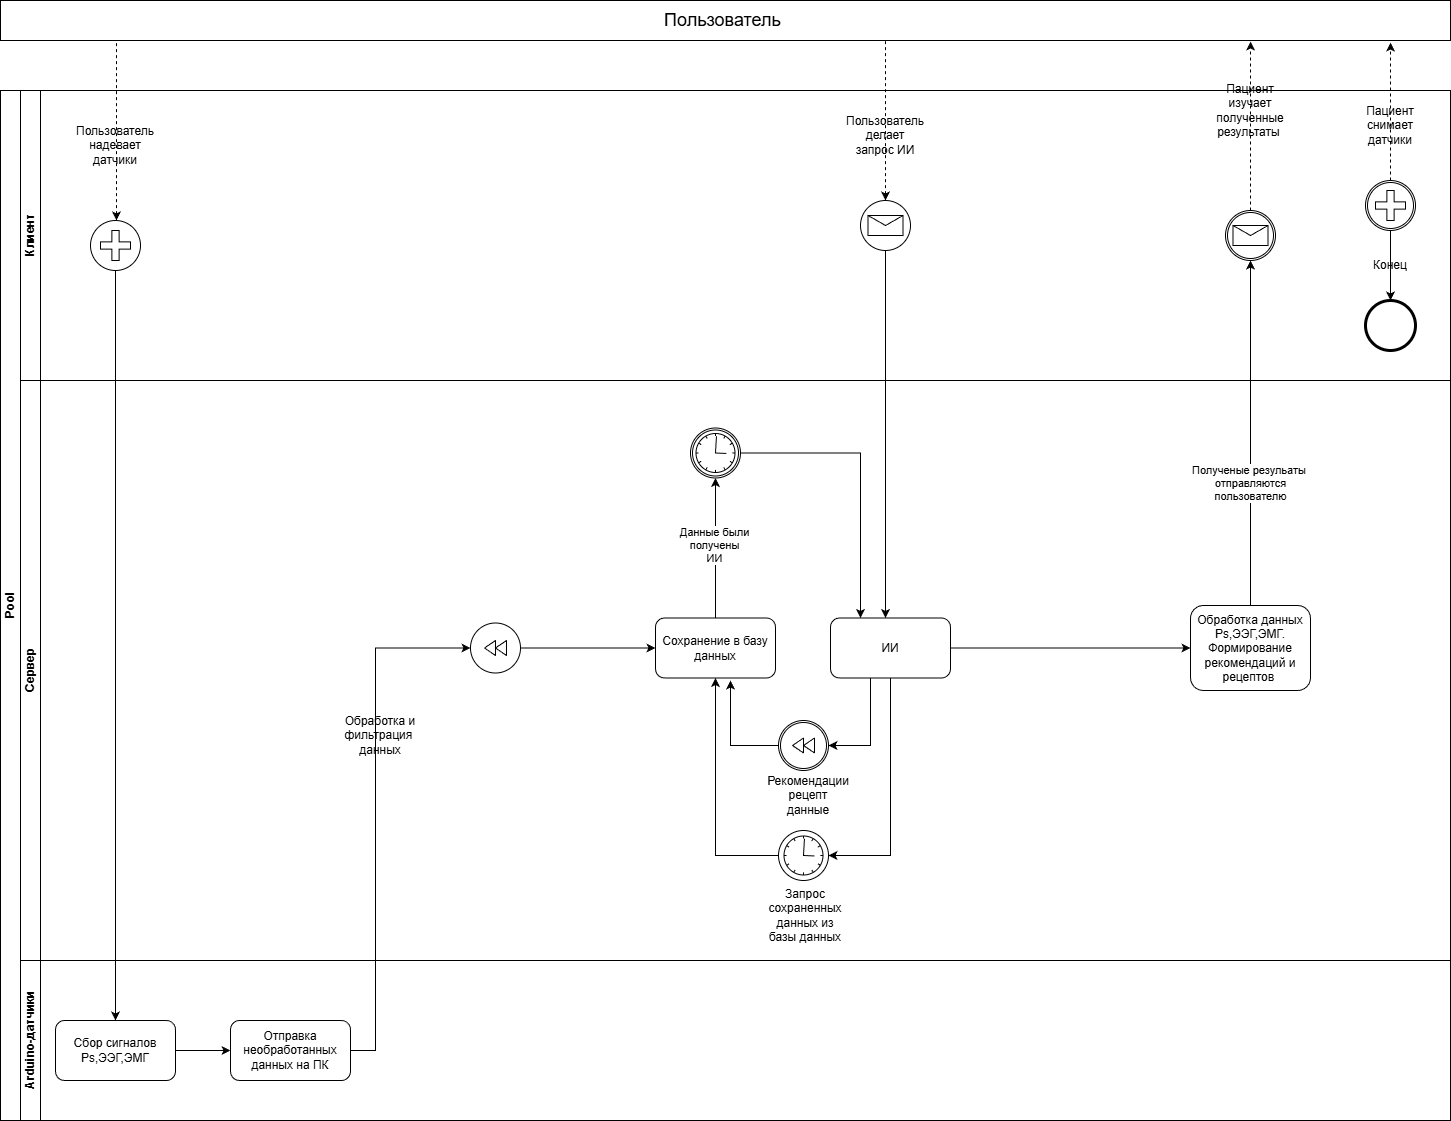
\includegraphics[width=0.9\textwidth,height=0.7\textheight,keepaspectratio]{images/bpmn.png}
\end{center}
\newpage


\gdef\ESKDtheSignature{ТПЖА.090301.838-02 ДПЛ}
\gdef\ESKDtheTitle{Схема взаимодействия модулей системы}
\begin{center}
  \vspace*{10mm}
  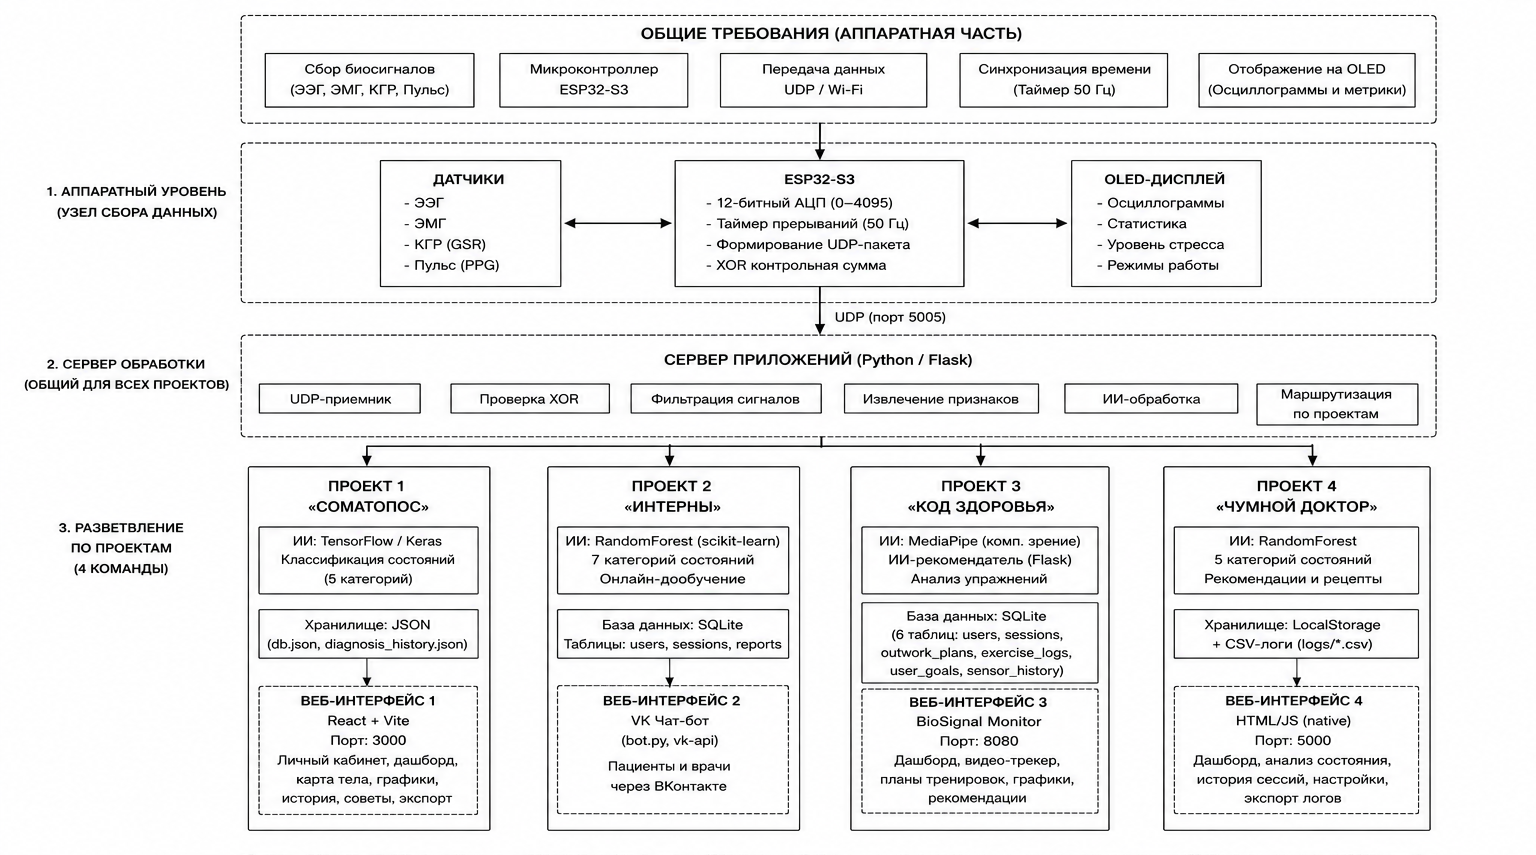
\includegraphics[width=0.9\textwidth,height=0.7\textheight,keepaspectratio]{images/complex_scheme.png}
\end{center}
\newpage

\gdef\ESKDtheSignature{ТПЖА.090301.838-03 ДПЛ}
\gdef\ESKDtheTitle{}
\begin{center}
  \vspace*{10mm}
  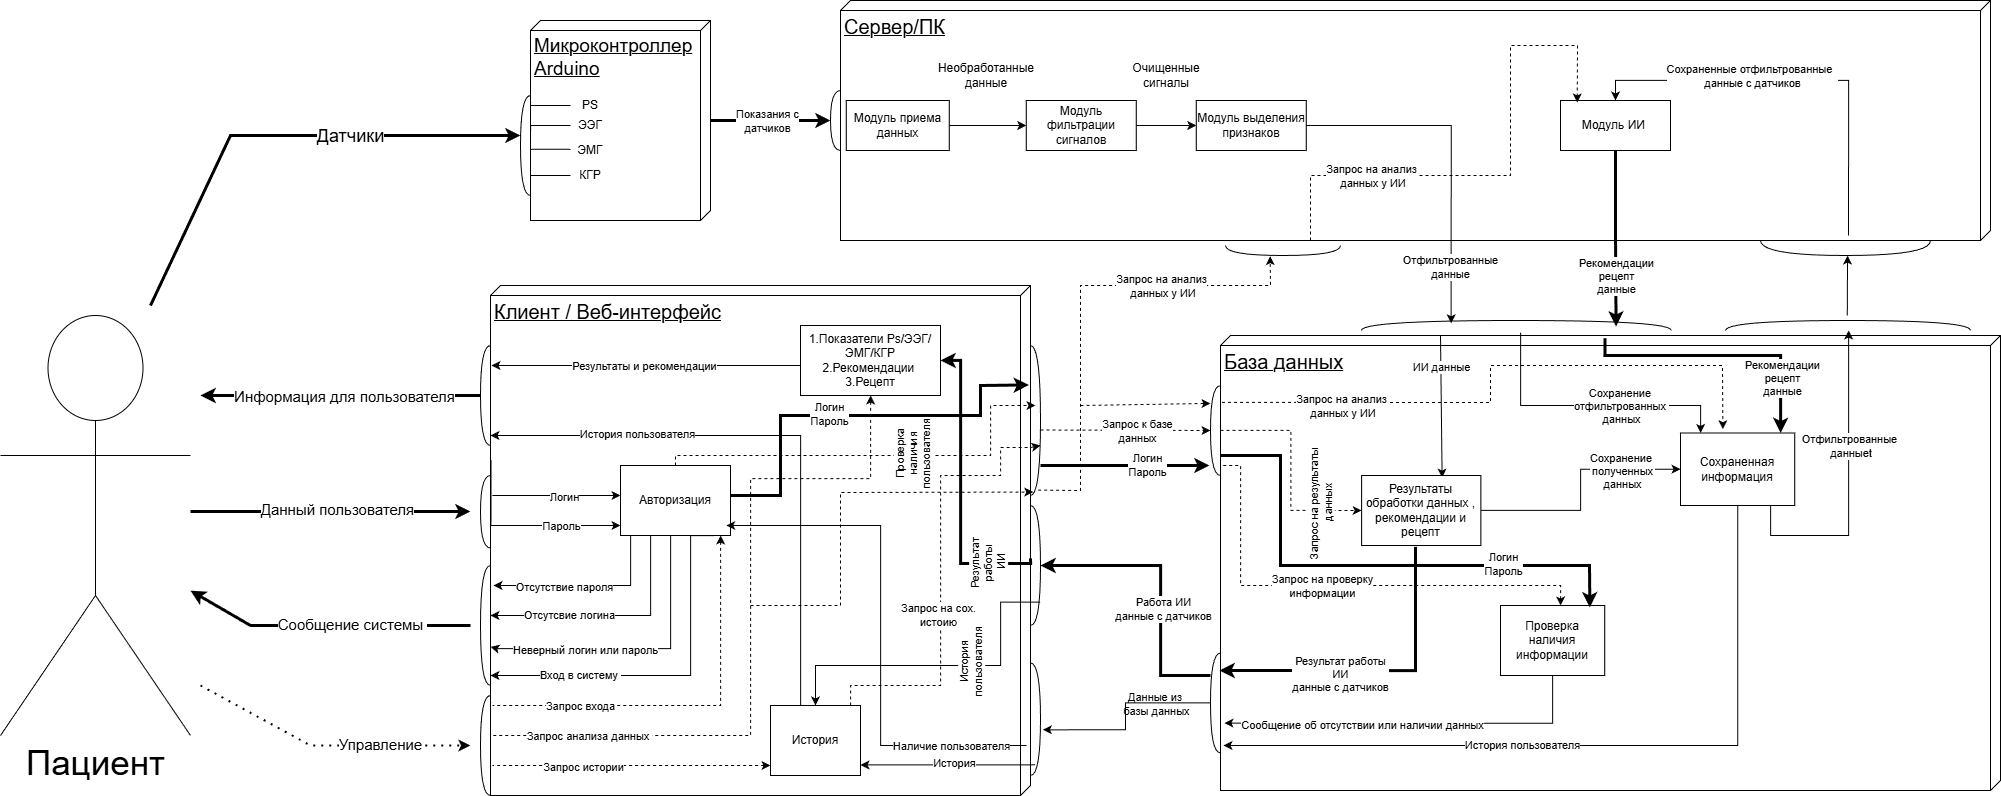
\includegraphics[width=0.9\textwidth,height=0.7\textheight,keepaspectratio]{images/диаграмма_разв.png}
\end{center}
\newpage

\gdef\ESKDtheSignature{ТПЖА.090301.838-04 ДПЛ}
\gdef\ESKDtheTitle{Схема электрическая принципиальна}
\begin{center}
  \vspace*{10mm}
  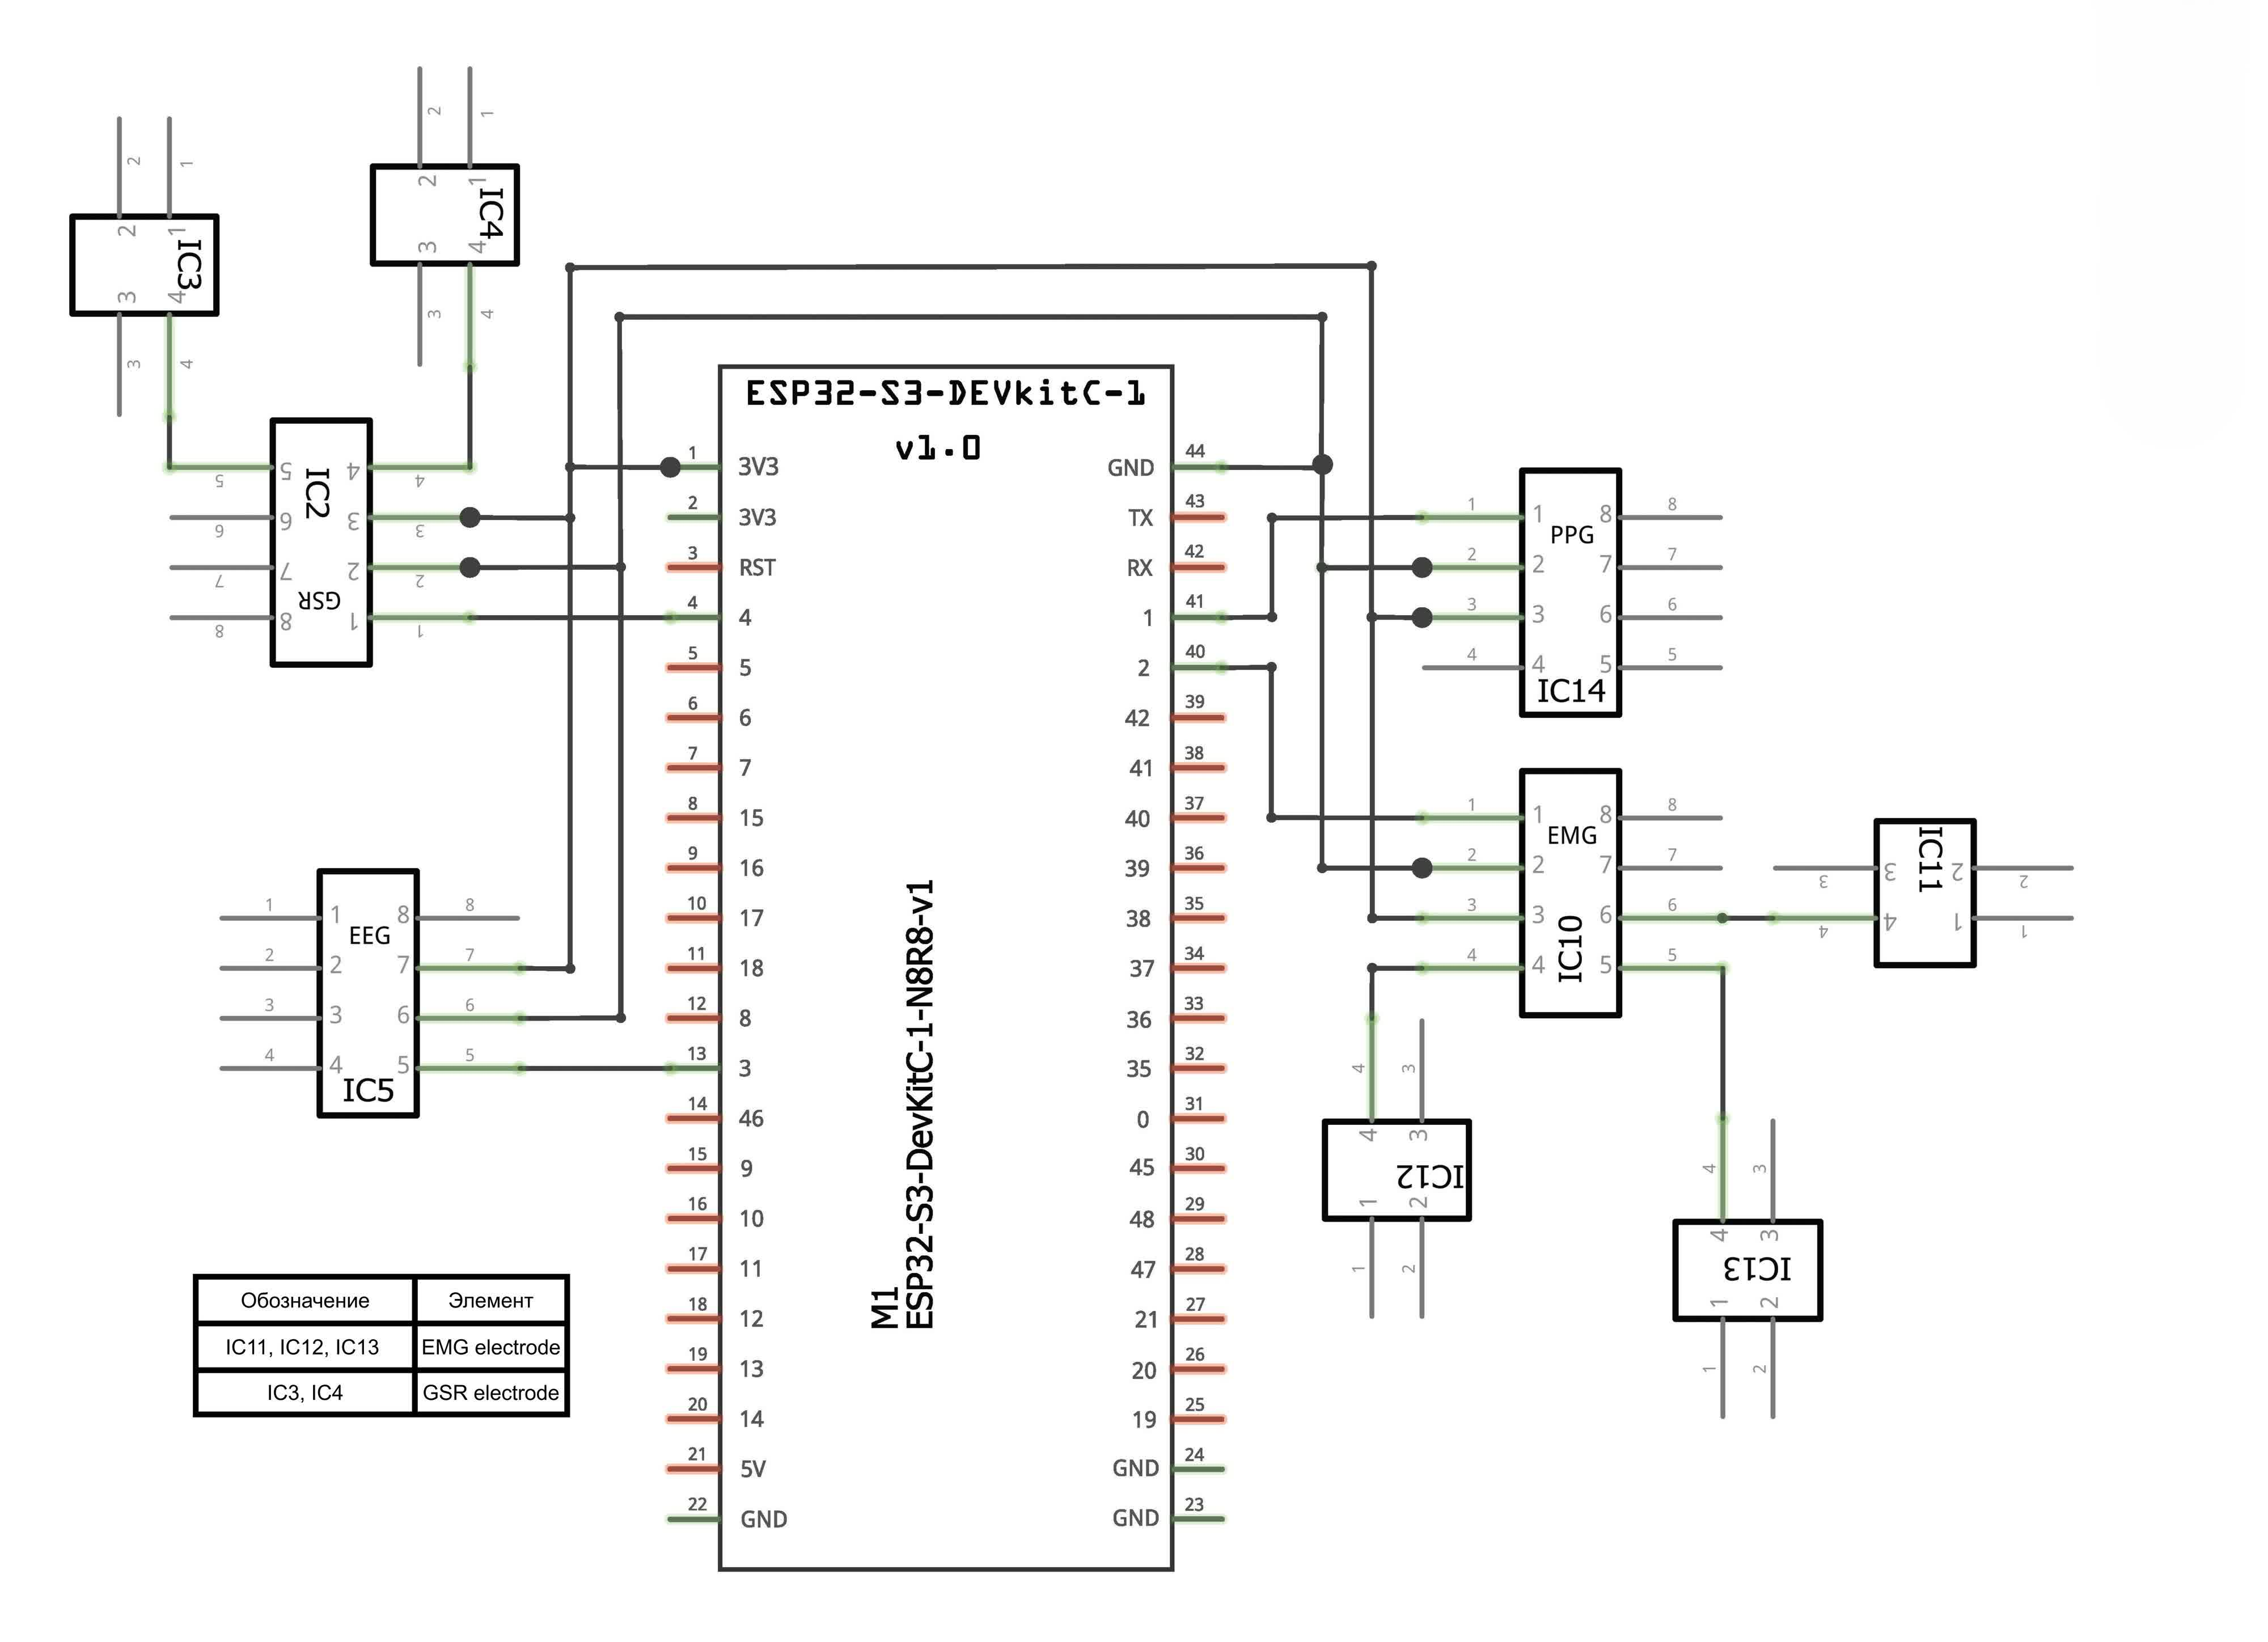
\includegraphics[width=0.9\textwidth,height=0.75\textheight,keepaspectratio]{images/Arduino_схема.jpg}
\end{center}
\newpage

\gdef\ESKDtheSignature{ТПЖА.090301.838-05 ДПЛ}
\gdef\ESKDtheTitle{Структура интерфейса}
\begin{center}
  \vspace*{10mm}
  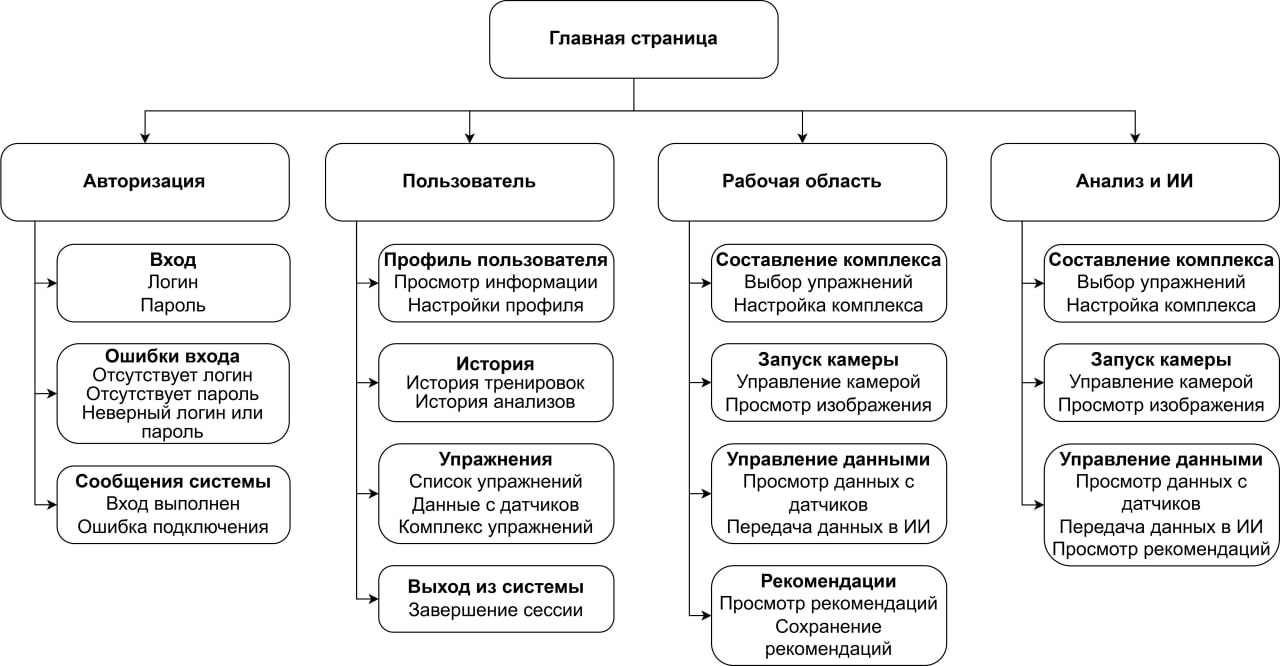
\includegraphics[width=0.9\textwidth,height=0.7\textheight,keepaspectratio]{images/interface.jpg}
\end{center}
\newpage

\gdef\ESKDtheSignature{ТПЖА.090301.838-06 ДПЛ}
\gdef\ESKDtheTitle{Схема функционирования устройства}
\begin{center}
  \vspace*{10mm}
  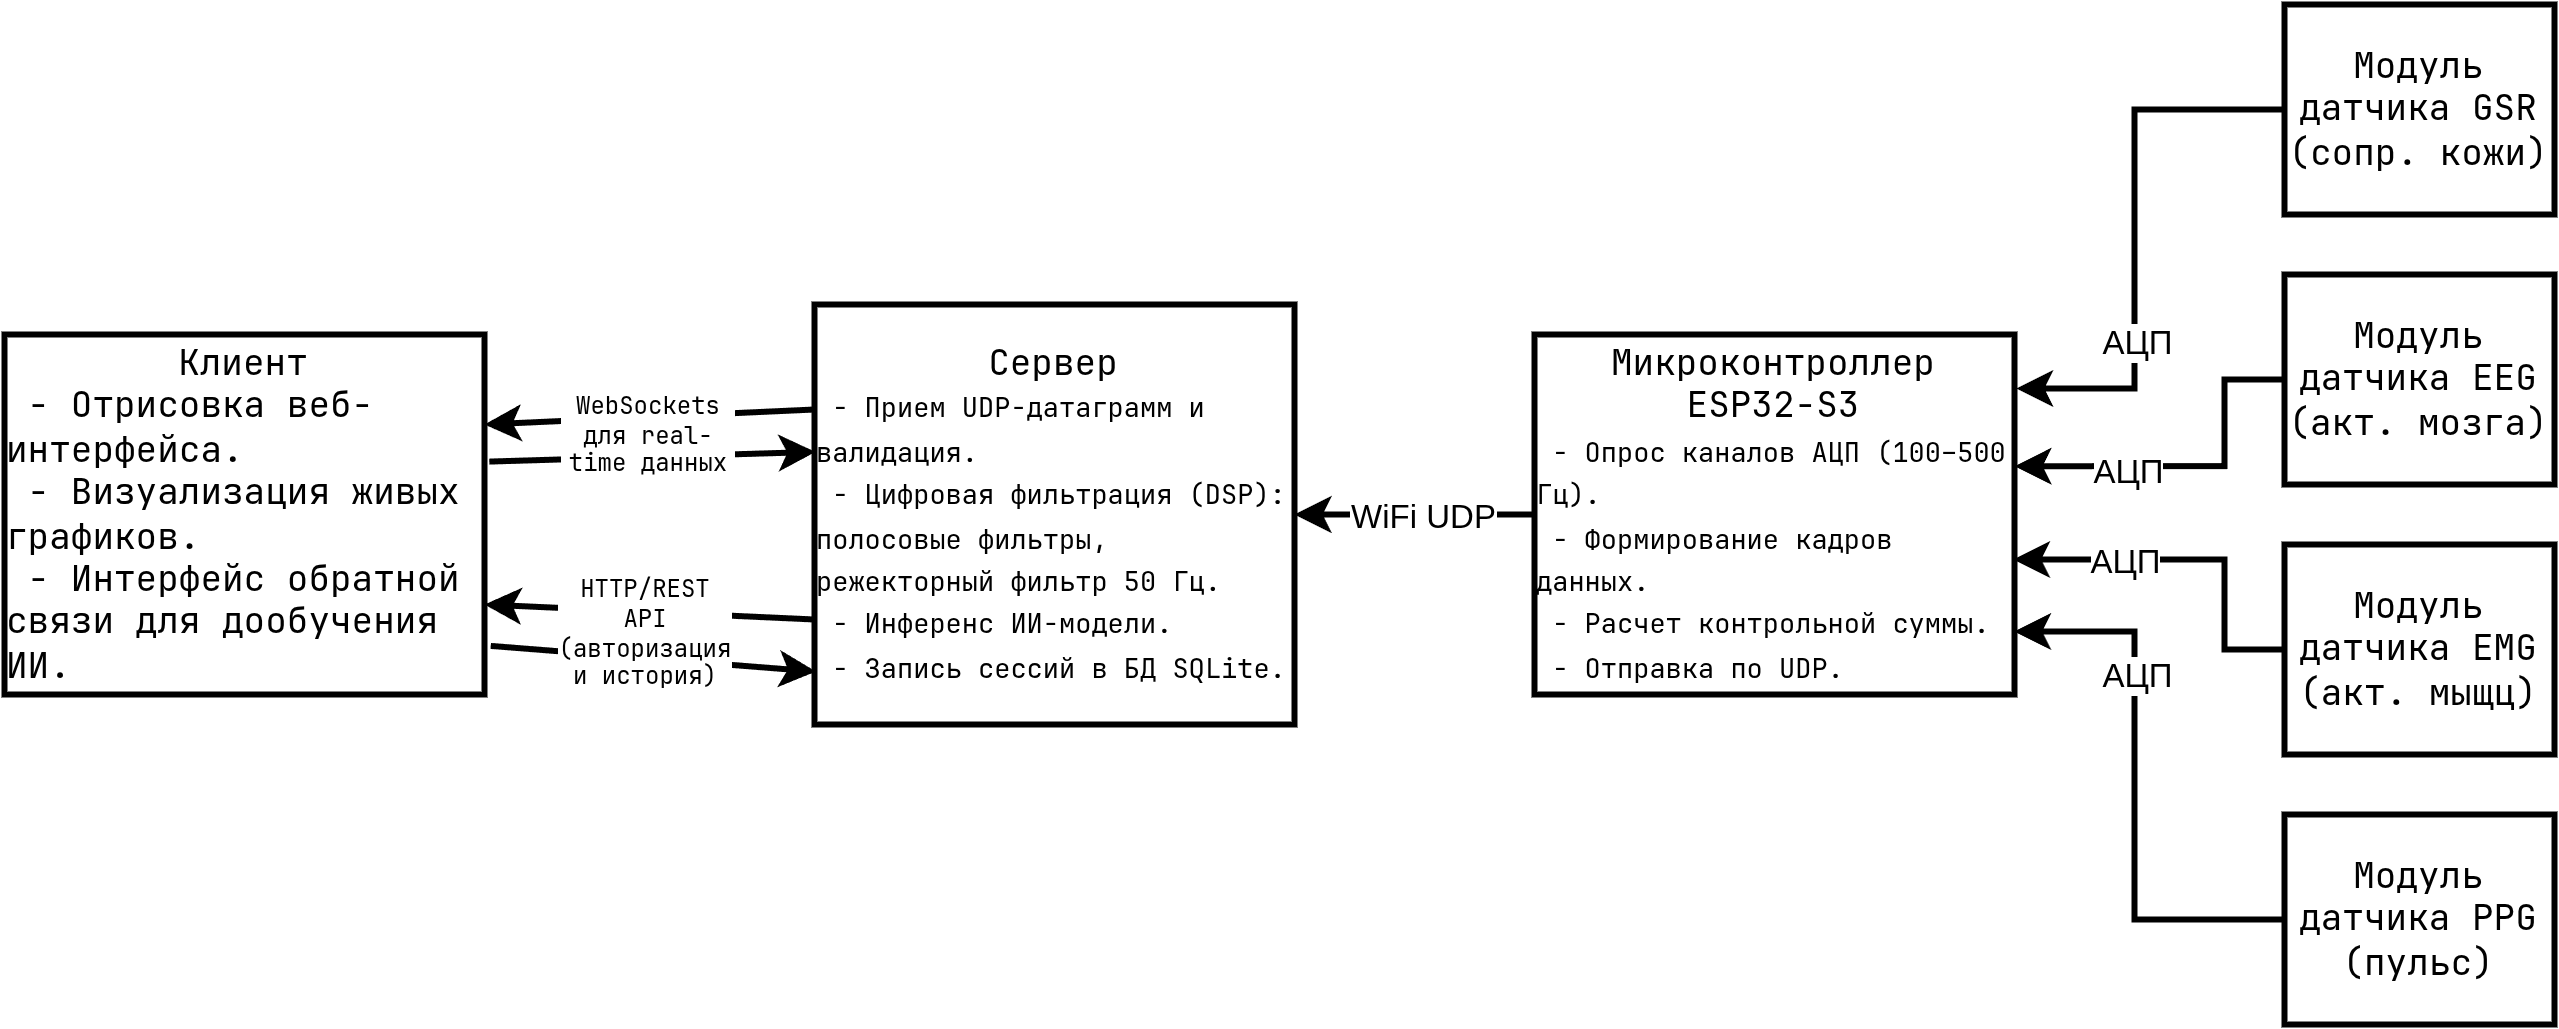
\includegraphics[width=0.9\textwidth,height=0.7\textheight,keepaspectratio]{images/funct_scheme.png}
\end{center}

\end{document}
